\chapter{Introduction}
\label{chapter1}

%\setlength{\epigraphrule}{0pt}
\epigraph{\textit{The moment you doubt whether you can fly, you cease for ever to be able to do it.}}{ -- J.M. Barrie, \textit{Peter Pan}}


% **************************** Define Graphics Path **************************
\ifpdf
    \graphicspath{{Chapter1/Figs/Raster/}{Chapter1/Figs/PDF/}{Chapter1/Figs/}}
\else
    \graphicspath{{Chapter1/Figs/Vector/}{Chapter1/Figs/}}
\fi

\section{Motivation}
The evolution of internet has been changing our daily life. According to a report by the Internet World Stats \cite{Internet1}, there is now more than 3 billions internet users, accounting for 40\% of the world's population. The number of internet users are increasing rapidly and also keep producing a huge amount of internet data. It is important to analyze these data because it can provide valuable information about our daily activities. Among many interesting problems that need to be investigated, recognizing event in internet videos has been drawing a lot of attention in recent years. 

Recognizing event refers to the process of automatically identifying video clips that contain a particular event of interest. This is a challenging problem because we need to build computer system to recognize event not only from video metadata but also from its content. The detail definition of this task and its challenges will be described in Section \ref{c1_problemdefinition} and Section \ref{c1_challenges} respectively. 

Event recognition technologies are mainly employed in \index{video retrieval} video retrieval systems to facilitate the retrieving progress. A video retrieval system that equipped such technologies can have numerous applications such as video search, video recommendation and video filtering. For example, below are some application scenarios:

\begin{itemize}
	\item \textbf{Video search.}\index{video search} This is an important function in most of video sharing websites. Most of the time, these websites only provide a search interface that supports text queries. However, in order to do that, videos must have already been indexed based on its content and other metadata. Using the provided interface, user can search for a specific tutorial such as ``how to make a cake'',  ``how to repair an appliance''; or some specific entertainment videos such as "a dog show" and "doing a magic trick".
	\item \textbf{Video recommendation.}\index{video recommendation} It is also very important for video sharing websites to recommend videos that may appeal to the user. The longer the user stay on their websites, the higher the benefit. The recommendation is often based on the user's favorite videos or recently watched videos. From these input videos, the system will search for similar videos through their database within a short time. For example, when the user watch a video of ``how to drive a car'', they may also expected to watch similar events such as ``how to park a car'' and ``common driving mistakes''.
	\item \textbf{Video filtering.} In contrast to video recommendation, video filtering is also an important application of event detection technologies. There are certain event that the managers do not want them to be public, especially when a government want to establish a video censorship. For example, videos that teach ``how to make a bomb'' or ``how to commit a suicide'' should be removed from the retrieval results. 

	Zillmann and Weaver \cite{JASP:JASP145} show that human tend to have violent responses when watching violent movies. In this case, event detection technology can be applied to filter out violent scenes \index{violent scene detection} in a movies. This technology has been employed in Facebook platform \cite{Internet3} to prevent the spread of a particular videos from over the internet. A video footage of a policeman being shot dead in the ``Charlie Hebdo shooting'' incident was among the first posts that were restricted by Facebook \cite{Internet3}. 
	
\end{itemize}

Motivated by these interesting applications, this dissertation aims to develop technologies for building an automatic event detection system. We will describe more about our research scope in the next section.

\section{Problem}
\label{c1_problemdefinition}
This dissertation addresses the problem of recognizing complex event in videos. Basically, it is the process of automatically identifying video clips that contain a particular event of interest. There are two important characteristics of our target problem. 

First, we are dealing with \textbf{complex event}. A complex event consists of various human activities and occurs in some particular settings. For example, ``changing a vehicle tire'' is an complex event that often happens at a garage or on street. This event contains several activities such as removing hubcap, turning lugwrench, unscrewing bolts and pulling rim out of tire. Complex event recognition differs from the traditional action recognition \index{action recognition} task in that it is the combination of multiple human actions or activities. It often contains various interactions between human and objects in different scenes. Therefore, a complex event video is often longer than a single action video. Moreover, action videos are often captured in controlled environment, while complex event videos are often recorded by internet users, which is uncontrolled or arbitrary environment. 

% % mentioned about CBVR 
Second, we are dealing with \textbf{multimedia data}. Internet videos can contain information from various mediums such as audio, visual and textual. Beside information from its content, internet videos often come with user-provided metadata description such as titles, tags and descriptions. Traditionally, videos are indexed and retrieved based on this metadata information. However, text-based video retrieval systems face an intrinsic limitation that is the semantic gap \index{semantic gap} between the content of the video and the information provided by the users. Moreover, this information is tend to be noisy and not always reliable. Therefore, we focus on utilizing multimedia data to build an effective event recognition system.

Due to the uncontrolled capturing condition of the complex videos, it is also interesting to know which parts of the video are important for recognizing event? How can we detect these parts? And suppose these parts do exist, how can we utilize them for complex event recognition? These challenging questions are also addressed in our dissertation.  

\section{Challenges}
\label{c1_challenges}
\begin{itemize}
	\item{\textbf{Large content variation.}} The large content variation refers to the diversity of a complex event. Even though an event only involve with some specific objects, activities and scenes, the variety among within these classes is also very high. For example, "birthday party" is a complex event. This event can be happen during day or night and set in indoor (a home, a restaurant) or outdoor (a backyard, a park) environment. Typically, in a birthday party, the presence of a birthday cake is of the utmost importance. However, in the real world setting, even the birthday cake can be very different from video to video. Figure \ref{c1_largecontent} shows some examples of birthday cake appear in internet videos. 
	\begin{figure}
		\centering
		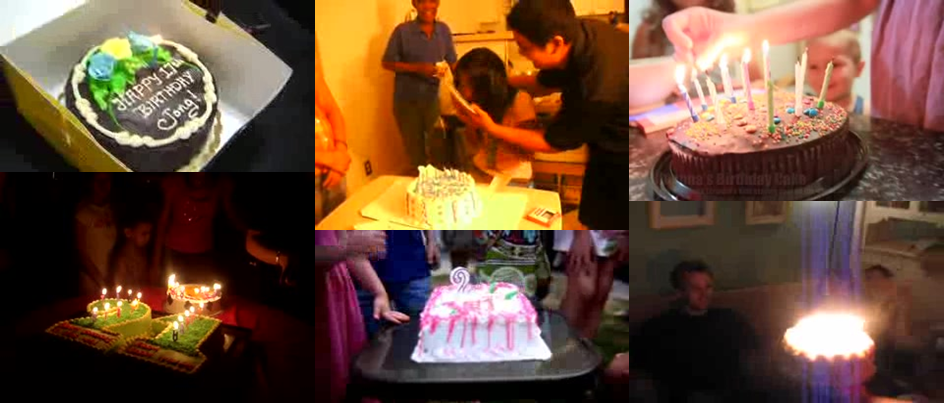
\includegraphics[width=1\textwidth]{largecontent.png}
		\caption{The large variation of birthday cake in the birthday party event.}
		\label{c1_largecontent}
	\end{figure}
	
	In terms of content variation, recognizing complex event is more challenging than other tasks such as instance search \index{instance search} or copy detection \index{copy detection}. The instance search task aims to search for a certain specific person, object or location. These instances can have different views but it must belong to the same target of interest in the real world. The target of copy detection task is a little bit more flexible. It aims to detect a video segment that is derived from another video. The copy video can be derived from the original video by means of transformations such as addition, deletion and modification. To this end, the complex event detection task has the utmost content variation.
	 
	\item{\textbf{Uncontrolled capturing condition.}} The uncontrolled capturing condition distinguish the complex event recognition task and the traditional action recognition task, which is often recorded in studio settings. As a result, techniques that work well for action recognition might no longer be effective for detecting complex event. For example, camera motion is one of the frequent prominence in internet videos. Although popular motion features \index{motion feature} such as \nomenclature[-stip]{STIP}{ Spatial-temporal Interest Points} STIP \cite{Laptev03space-timeinterest} and \nomenclature[-hog3d]{HOG3G}{Histogram of 3D Gradients} HOG3D \cite{Klaser08BMVC} can effectively recognize action in studio videos, it shows limited performance in internet videos because it is not designed to handle camera motion. On the other hand, Dense Trajectories proposed by Wang takes into account the camera motion and demonstrates superior performance.
	 
	One of the direct consequence of uncontrolled capturing condition is that user-generated videos often contain irrelevant information to the event of interest. In other words, different parts of the video have different levels of relatedness to a particular event. This leads to a challenging problem which is how to discard irrelevant information from the video representation. It is especially difficult when the annotation of each part of the video is almost not available. Figure \ref{c1_uncontrolled} shows some examples of noisy information in internet videos.
	
	\begin{figure}
		\centering
		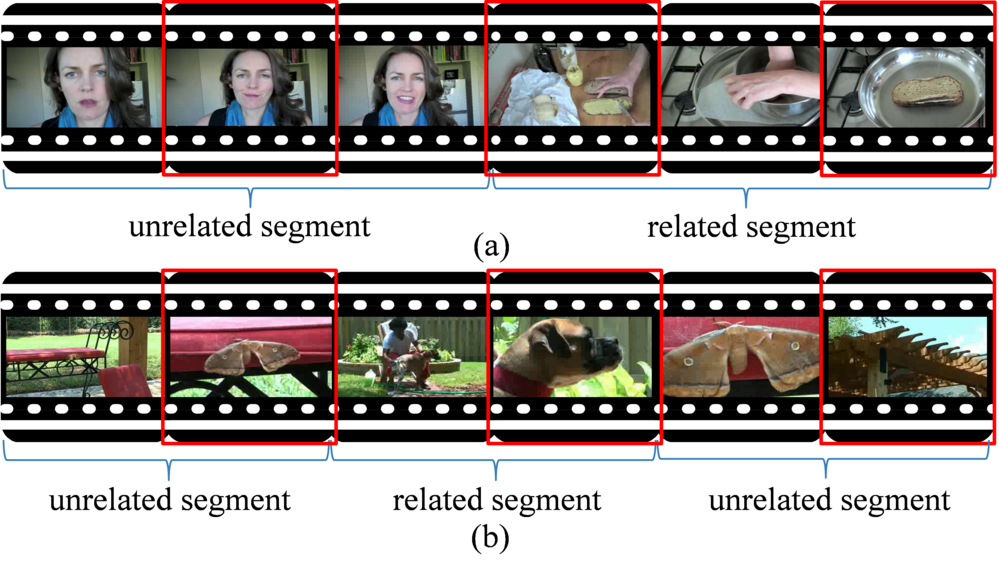
\includegraphics[width=1\textwidth]{teaser_image.png}
		\caption{(a) Example video for ``making a sandwich'' event: the related segment appears after a self-cam segment (unrelated); (b) example video for ``grooming an animal'' event: related segment is sandwiched between two unrelated segments. This kind of video is popular in realistic video datasets like MED. The frames with a red outlined box are examples of the extracted keyframes when using a keyframe-based approach, which suffers from both noise and missed extraction.}
		\label{c1_uncontrolled}
	\end{figure}
	 
	\item{\textbf{Near-miss videos.}} Near-miss video refers to a kind of video that is closely related to a particular event, however, it is not a positive instance of that event. Because a complex video is often composed by several objects or activities in some particular order, it might not be considered an event video if there is a lack of certain evidences. So a near-miss video can contain several evidences but not enough to define an event. This property of near-miss video often harm the performance of an event detection system. In fact, this kind of video is also prevalent in the setting of complex event recognition task. For example, ``Changing a vehicle tire'' is a complex event that involve one or more people to replace a tire on a vehicle. An event is not defined if the tire of the vehicle is not replaced. Examples of near-miss videos can be seen in Fig. \ref{c1_nearmiss}.
	
	\begin{figure}
		\centering
		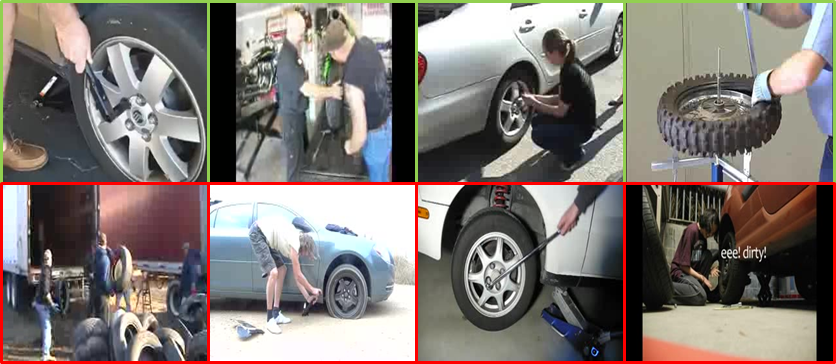
\includegraphics[width=1\textwidth]{near_miss.png}
		\caption{Example of near-miss video for ``Changing a vehicle tire'' event. The first row shows some positive videos. The second row shows near-miss videos, which is very easy to be confused with positive ones, even for human.}
		\label{c1_nearmiss}
	\end{figure}
		
	\item{\textbf{Large scale video database.}} Last but not least, we have to deal with big data as well. We have to accurately search for a particular event through a large video archive in a reasonable amount of time. In some complex event detection task such as \nomenclature[-trecvid]{TRECVID}{TREC Video Retrieval Evaluation} TRECVID Multimedia Event Detection (MED) \nomenclature[-med]{MED}{Multimedia Event Detection}, the evaluation time is also limited, which forces the participants to care about the efficiency of their systems.
	
\end{itemize}

\section{Contributions}

We made following contributions:

\begin{itemize}
\item We propose using a segment-based approach to overcome the limitations of  the video-based approaches. The basic idea is to examine shorter segments instead of using the representative frames or entire video. We carry thorough experiments to verify our proposed method by investigating different strategies to decompose a video into segments. These strategies include uniform segment sampling and segments based on shot boundary detection.

\item We propose a new video pooling strategy, called sum-max video pooling, to deal with noisy information in complex videos. This pooling technique is based on the layer structure of video. Basically, we apply sum pooling at the low layer representation while using max pooling at the high layer representation. Sum pooling is used to keep sufficient relevant features at the low layer, while max pooling is used to retrieve the most relevant features at the high layer, therefore it can discard irrelevant features in the final video representation. 
	
\item We propose a new method, named \nomenclature[-edmil]{EDMIL}{Event-driven Multiple Instance Learning} Event-driven Multiple Instance Learning (EDMIL), to learn key evidences for complex event detection. We treat each segment as an instance and model it in a multiple instance learning framework \cite{andrews2002support}, where each video is a "bag". The instance-event similarity is quantized into different levels of relatedness. Intuitively, the most (ir)relevant instances should have higher (dis)similarities. Therefore, we propose to learn the instance labels by jointly optimizing the instance classifier and its related level.
	
\end{itemize}

\section{Thesis Overview}

%\nomenclature[g-pi]{$\pi$}{ $\simeq 3.14\ldots$} to be listed after $\alpha$\nomenclature{$\alpha$}{The first letter of the greek alphabet} \index{MED}

The remaining of this dissertation is organized as follows:

Chapter \ref{chapter2} introduces some background that is related to our research. This background encompasses an introduction to TRECVID MED task and dataset. It also provide basic knowledge about some low level features and feature encoding methods, which is necessary to re-implement our system. 

Chapter \ref{chapter3} presents our segment-based approach for complex event detection. At first we introduce the video-based approach and some of its limitation. After that we present the segment-based approach with several strategies to decompose a video into segments.

Chapter \ref{chapter4} presents our sum-max video pooling for complex event recognition. At first we introduce the layer structure of a video. Based on this layer structure, we propose a new video pooling technique which is a combination of sum pooling and max pooling.

Chapter \ref{chapter5} presents our method to detect event using the evidential description of an event. We also present a method to calculate the similarity between a video segment and an event based on textual description. This method can also provide evidences for event detection.

Chapter \ref{chapter6} concludes this dissertation by summarizing our contributions and discussing about the future work.

	\begin{figure}
		\centering
		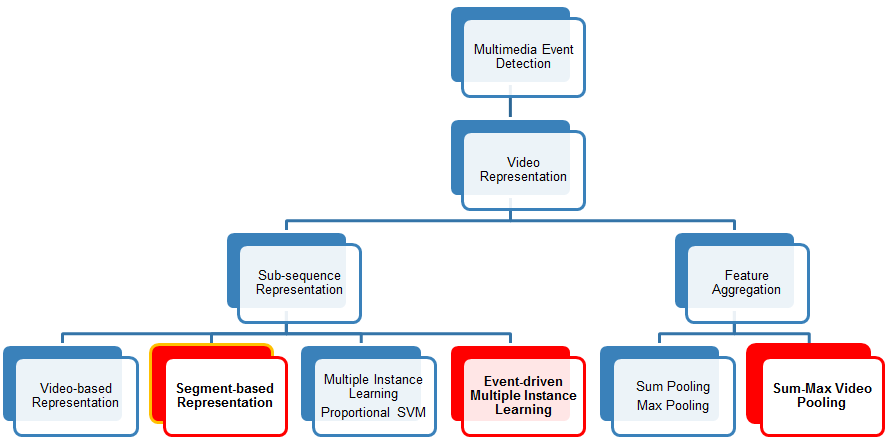
\includegraphics[width=1\textwidth]{outline.png}
		\caption{Outline of our thesis. Our contributions are highlighted in red boxes.}
		\label{c1_outline}
	\end{figure}
	
\nomenclature[-sb]{SB}{Segment-based}
\nomenclature[-sm]{SM}{Sum-Max Video Pooling}
\nomenclature[-map]{MAP}{Mean Average Precision}
\nomenclature[-map]{SBD}{Shot Boundary Detection}

